\documentclass[a4paper]{article}

\usepackage[english]{babel}
\usepackage[utf8]{inputenc}
\usepackage{amsmath}
\DeclareMathOperator*{\argmax}{argmax}
\usepackage{graphicx}
\usepackage[colorinlistoftodos]{todonotes}
\usepackage[nottoc]{tocbibind}




\begin{document}

\begin{titlepage}
	\begin{center}
		
		
\includegraphics[width=0.8\textwidth]{NTU.png}
		\vspace{2cm}
		
		\huge
		
		\textbf{Pricing problems with \\Thompson Sampling}
		
		\vspace{1cm}
		\Large
		Lee Wai Leong Samuel
		
		\vspace{2cm}
		\Large
		Nanyang Technological University\\
		School of Physical and Mathematical Sciences\\
		8 April 2019
		
		\vfill
		
		Final Year Project\\
		Supervisor: Dr. Yan Zhenzhen
		
		\vspace{0.8cm}
		
	\end{center}
\end{titlepage}

\begin{center}
%	\renewcommand{\baselinestretch}{1.5}
	\large
	\textbf{Acknowledgements}
	\vspace{1cm}
	
	My heartfelt thanks and gratitude go to Dr. Yan Zhenzhen for her patience and guidance throughout the project. There were times when I felt lost and was on the verge of giving up but she has been extremely understanding and encouraging. I have learned and grown a lot both technically and personally from her knowledge and enthusiasm on this topic. It has been a great privilege to have her as my thesis supervisor.
\end{center}
\pagebreak
\begin{center}
%	\renewcommand{\baselinestretch}{1.5}
	\large
	\textbf{Abstract}
	\vspace{1cm}
	
	
	In 1933, William R. Thompson proposed an algorithm known as Thompson sampling in order to maximise culmulative payoff in a multi-armed bandit (MAB) problem. MAB problems have been frequently used to model real-life decision making scenarios. This paper explores the extension of Thompson sampling to other problems beyond the MAB setting. More specifically, Thompson sampling is applied to product sales using data from a real dataset in a dynamic pricing setting as part of the multi-product pricing problem. 
\end{center}
\pagebreak
\large
\renewcommand{\baselinestretch}{1.5}
\tableofcontents



\pagebreak
\section{Introduction}
\subsection{Problem description}
With sales reaching 10\% of total global sales, there is little doubt that e-commerce is a very popular online activity \cite{nano3}. It is expected to continue growing to 15\% in 2020 which has led to many firms setting up their own e-commerce portals or through other e-commerce giants. In order to differentiate themselves from the competition, most firms implement some sort of sales promotion. Some examples of promotions include percentage discounts (X\% off), flat amount discounts (\$X dollars off), BOGO (Buy one get one at X\% off) and multi-buys (2 for the price of 1).  In a ``full-cut promotion", there is usually a pre-determined amount. For each time an order satisfies the pre-determined amount, it would be eligible for a flat amount discount. For example, Calvin Klein recently had the promotion ``For every \$100 spent, enjoy \$40 off" on their website \cite{CK}. Although sales promotions like these are mainly used for clearing excessive stock, they do have many other benefits such as customer attraction and increasing short-term revenue. It would thus be valuable to study pricing problems with sales promotions as they are implemented very frequently in e-commerce. 


\subsection{Literature review}
In order to study full-cut promotions, the multi-product pricing problem should first be investigated as it is a more fundamental problem of dynamic pricing problems. In this area, work has been done in the cases of known demand function and unknown demand function. In the former case, the dynamic pricing problem is typically modelled as the multi-armed bandit (MAB) problem and is solved by well-known methods such as the upper confidence bound (UCB) algorithm. Bubeck \& Cesa-Bianchi (2012) summarised this problem without resource constraints in their paper. Badanidiyuru et al. (2013) further improved on this approach by adapting the UCB algorithm to a MAB problem with resource constraints as such constraints cannot be easily modelled in the typical MAB problem. This was achieved by maintaining a vector of costs and adjusting it by combining confidence bounds and multiplicative updates. 
\newline
\newline
In the latter case of unknown demand function, Aviv \& Pazgal (2005) used a certainty-equivalent heuristic to obtain an approximate pricing solution in a partially observed Markov decision process (POMDP) framework. Both Araman \& Caldentey (2009) and Farias \& Van Roy (2010) extended on this approach by proposing more sophisticated approximate dynamic programming heuristics. Araman \& Caldentey (2009) used a sequence of models with varying levels of complexity to model the demand in which the underlying process followed a Poisson distribution, and then proposed a set of algorithms that efficiently approximated the solution. Similarly, Farias \& Van Roy (2010) also used a Poisson distribution for their model but with a different heuristic approach which they called \textit{decay balancing.} Broder \& Rusmevichientong (2012) used maximum likelihood estimation to obtain pricing policies under a general parametric choice model and also when the family of demand functions satisfied a ``well-separated" condition. 
\newline
\newline
The main objective of this paper is to apply Thompson Sampling to solve the dynamic pricing problem under sales promotions. We first compare the results of Thompson Sampling with other popular algorithms in a MAB problem before moving to the dynamic pricing setting with data from a real dataset where there are infinite arms.
\newline
\newline
Dynamic pricing involves a seller regularly adjusting the prices of products in order to obtain information about the products' demand, and then exploiting this information in order to maximise revenue. While many other efficient algorithms exist to solve MAB problems, Thompson sampling was chosen as it has been shown to be highly competitive with promising performance \cite{thomp}. 

\section{Description of approaches}
\label{sec:approach}
The first approach would be to use the classical Thompson sampling algorithm in a MAB problem where each price vector represents an arm. In this approach, there is a finite number of price vectors and the goal is to learn the demand distribution and expected payout of each price vector so as to maximize revenue over time. In this approach, we assume the demand function to be a multinomial-logit (MNL) model.
\newline
\newline
The second approach would be to use Thompson sampling in a dynamic pricing algorithm. More specifically, we apply the Thompson Sampling algorithm for dynamic pricing proposed by Ganti, Sustik, Tran \& Seaman (2018). Their algorithm works as follows: a Bayesian prior is initialised on unknown parameters using historical data. The posterior is obtained via Bayes rule and a sample is taken from this posterior as an estimate of parameters. A new set of prices (likely to be different from the previous time step) is obtained by maximising a reward function with the sampled parameters. This process will continue until the end of all time periods. In this approach, there is usually a larger set (possibly infinite) of price vectors in contrast to the MAB setting which only has fixed price vectors. The goal is to learn the distribution of the price elasticity of each product in order to maximise revenue and not the distribution under each price vector. The demand function is assumed to be a modified constant elasticity function which will be explained in greater detail later.

\section{Analysing a dataset with promotions}
The given data is sales data of 66 products (children's books) sold over a period of 11 days without any changes in price while under some sales promotion from an e-commerce firm based in China. We will use this dataset in our second approach. The dataset contained 4716 rows and 23 columns. Each row represented a product in an order that was placed while each column represented a feature of each order such as order ID, order date, user ID, goods ID, price and quantity.
\newline
\newline
It is known that there is an ongoing sales promotion in the data in which an order would be eligible for discounts by fulfilling a minimum value. This value is defined as the threshold. For example, every \$99 spent would be eligible for a \$50 discount. One possible method to find the threshold would be through trial and error.
\newline
\newline
If $X$ is trialed as the threshold value, orders can be categorized into groups of different multiples of $X$. The first group would consist of orders ranging from \$0 to \$($X$-1) and the second group would range from \$$X$ to \$2$X$-1 and so on. The mean discount for each group can then be calculated. If $X$ is the threshold value, the mean discount for the first group should be 0 as all orders in that group should not have fulfilled the minimum amount. Likewise, the mean discount for subsequent groups should be multiples of the discount. Plotting the mean discounts for each group should reveal a linear relationship.
\newline
\newline
For this data set, multiple values of $X$ (80, 90, 99, 110, 120) were tested and the mean discounts were plotted in Figure \ref{fig:cut}. For $X = 80, 110$ and $120$, the gradients are not constant over each group. This suggests that some groups contain orders that qualify for different discounts from the rest. The plots of $X = 90$ and $X = 99$ indicate a strong linear relationship. However, at $Groups = 3$, the plot of $X = 90$ is not as linear as $X=99$. Thus, it is likely that the true threshold value of this data set is 99.

\begin{figure}
	\centering
	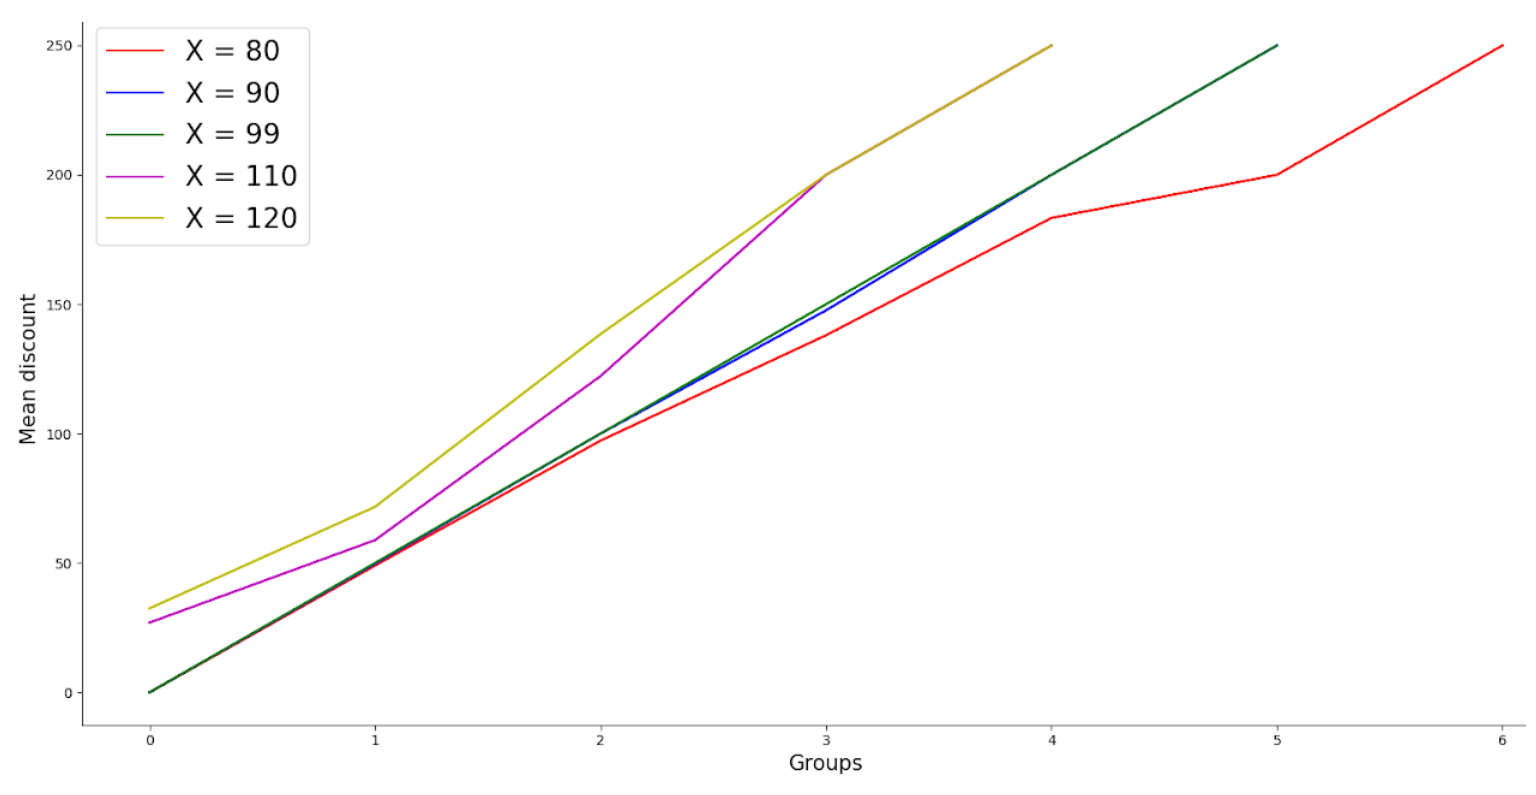
\includegraphics[width=1\textwidth]{cut.png}
	\caption{\label{fig:cut}Plotting mean discounts for each group}
\end{figure}

\section{First approach}
As mentioned earlier, we do not use the given dataset in this approach. Instead, we use the MNL model as our demand function.
\newline
\newline
In this approach, we use the classical Thompson sampling algorithm in a typical MAB problem. We compare the performance of the algorithm to the best possible outcome before comparing with other well known algorithms.

\subsection{Data generation}
The set of prices in the data set was used as one price vector. Two other price vectors were created by $\pm 10\%$ to the original price vector. Together, we may identify the 3 price vectors as lower price vector, middle price vector and higher price vector where the lower price vector is 10\% less than the middle price vector. The method described below was used to create simulation data.
\newline
\newline
For each price vector $k$, 1 data point was created using the MNL formula below and it represents the mean of the true demand under that price vector
\[X_{ik} = \frac{e^{V_i - P_{ik}}}{\sum_{j=0}^{N}e^{V_j - P_{jk}}} \tag{1}\]
where $V_i$ represents the customer's valuation of product $i$ and $P_{ik}$ is the price of product $i$ under price vector $k$. Thus, $X_{ik}$ is the mean of the true demand for product $i$ under price vector $k$. In the denominator, $j=0$ represents the option where the customer chooses not to buy anything and $N$ is the total number of products.
\newline
\newline
As there are now 3 price vectors, the valuation vector $V$ can be created by randomly sampling from a 5\% neighbourhood of $\hat{P}$ where $\hat{P}=\sum_{k=1}^{3}P_k$. $V_0$ is randomly sampled from the interval $(0,5).$
\newline
\newline
With the $V$ and $P$ vectors defined, the theoretical $X_i$ corresponding to each price vector can be created and they will represent the true demand. In the long run, the expected value of all data points for each price vector should be equal to the theoretical $X_i$.
\newline
\newline
For each price vector, 20 data points were created as historical data in order to obtain our prior distribution. In order to ensure that the expected value of all data points was equal to the theoretical $X_i$, 10 epsilon vectors were created and the data points were obtained by adding and subtracting the epsilon vector from the theoretical $X_i$. This process was repeated for the other two price vectors as well. In total, there were 60 data points created with each price vector having 20 data points.

\subsection{Implementation of classical TS}
In this approach, the objective was to learn the true demand function under each price vector. It was assumed that the true demand functions followed normal distributions. The prior distribution for each price vector was then estimated from the 20 data points generated earlier using maximum likelihood estimation. 
\newline
\newline
For iterations $t = 1,...,T$, the following process was done:
\begin{enumerate}
	\item A random sample was taken from each price vector's prior distribution.
	\item The estimated revenue under each price vector was calculated by multiplying the random sample and the price vector since each random sample represents the estimated demand under that price vector.
	\item The price vector with the highest estimated revenue was chosen as the selected arm for this iteration.
	\item The selected arm was pulled. The observed demand would be that price vector's theoretical $X_i$.
	\item The observed revenue was calculated by multiplying the observed demand with the price vector and also accumulated over all iterations.
	\item The observed demand was added as an observation to the selected arm's $H_{t-1}$ data points where $H_{t-1}$ is the number of data points under that price vector in the previous iteration.
	\item The prior distribution of that price vector was re-estimated with the $H_{t-1} + 1$ data points using maximum likelihood estimation.
\end{enumerate}
%\newline
%\newline
The number of times each price vector was selected was recorded. The price vector that was selected the most often would then be the arm with the highest revenue.
\newline
\newline
In order to validate that the chosen arm in the above process was the correct arm, a simple check was conducted for each arm. In each check, the same arm was chosen in every iteration and the observed revenue was cumulated. The arm with the greatest cumulated revenue would then be the theoretically correct arm. The average result of 10 initialisations of this approach over 1000 iterations is shown in Figure \ref{fig:one}. $T$ was set to be 1000 in order for us to observe any long term effects.
\begin{figure}[h]
	\centering
	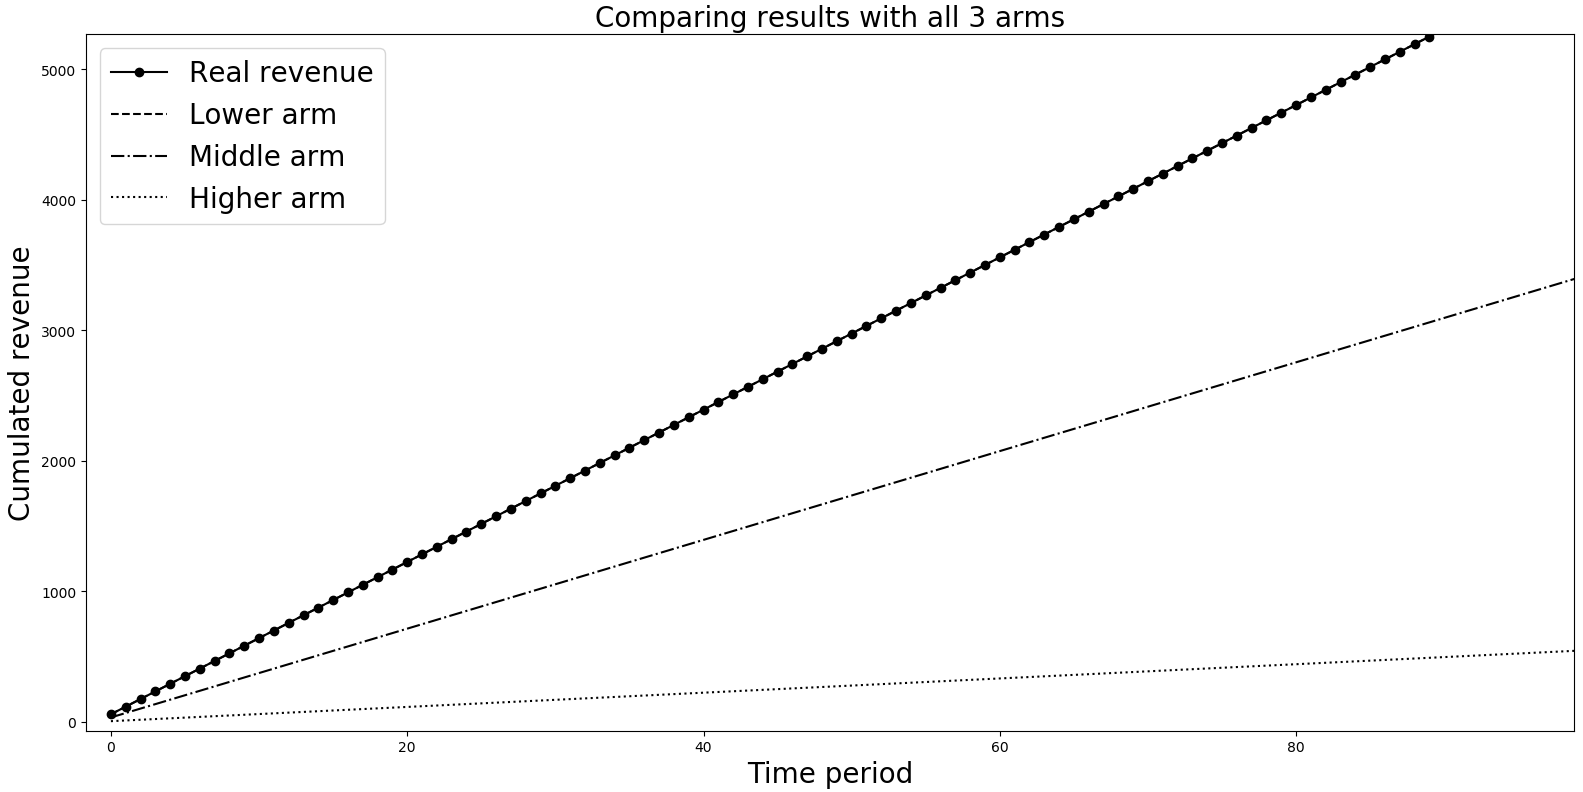
\includegraphics[width=1\textwidth]{Figure_1-2.png}
	\caption{\label{fig:one}Comparing revenue between all 3 arms and actual revenue}
\end{figure}
\newline
\newline
The dashed, dashed-dotted and dotted lines correspond to checks for each arm and they represent the true revenue under that arm. The solid line with circles represents the revenue under classical TS and interestingly, it has the exact same values as the lower arm in every iteration which is why the lower arm cannot be seen. Since the lower arm has the highest cumulated revenue out of all three arms, it is the theoretically correct arm. This means that Thompson sampling has already correctly identified the best arm right from the beginning and was exploiting it in every iteration.

\subsection{Comparison with other algorithms}
As mentioned earlier, the MAB problem is not new and many algorithms have been developed to solve it. Here, we compare the performance of Thompson sampling to other well-established algorithms in the same setting as the previous subsection. The algorithms we'll compare to are:
\begin{enumerate}
	\item Upper Confidence Bound - UCB1
	\item Upper Confidence Bound Tuned - UCB1-Tuned
	\item Epsilon-greedy algorithm
	\item Epsilon-greedy with optimistic initialisation
	\item Epsilon-greedy with decay	
\end{enumerate}
%\newline
%\newline
According to Figure \ref{fig:two}, the performance of the algorithms are all very similar in the beginning. The epsilon-greedy algorithm even manages to match TS until the 7th time period. However, if we observe the results at the end of the horizon in Figure \ref{fig:three}, the epsilon-greedy algorithms perform significantly poorer than TS. Unsurprisingly, greedy algorithms do not work well in most situations. UCB algorithms have been widely considered to be good solutions to MAB problems. From this example, we see that TS also outperforms them although to a smaller extent. This is probably because TS assumes a prior distribution from historical data while UCB does not, and instead requires the pulling of every arm (including suboptimal ones) at least once in the beginning which contributes to increased regret.
\begin{figure}[h]
	\centering
	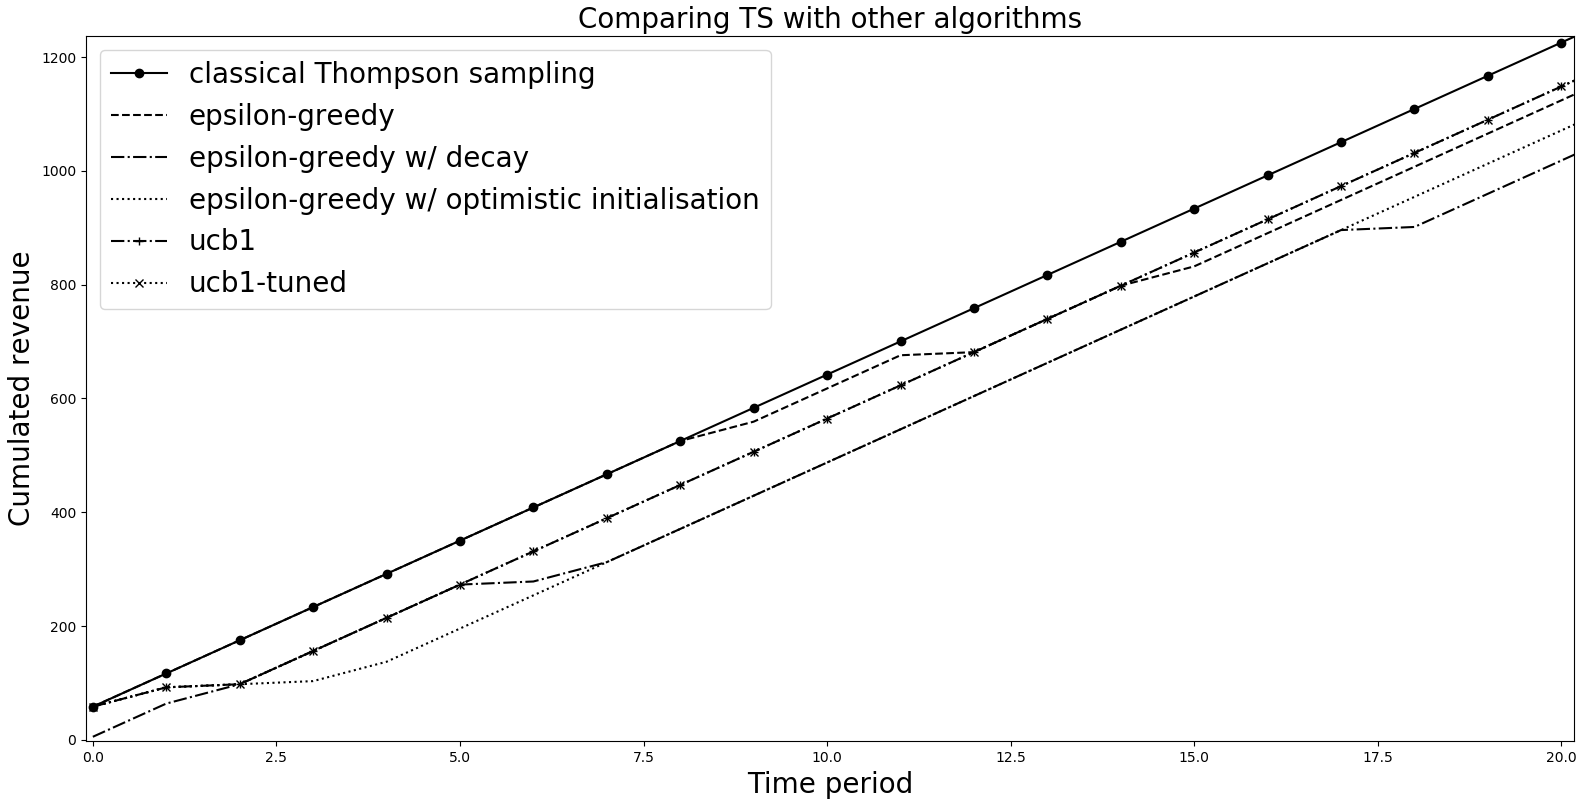
\includegraphics[width=1\textwidth]{Figure_1-3.png}
	\caption{\label{fig:two}Comparing revenue between all algorithms - first 20 time periods}
\end{figure}
\begin{figure}[h]
	\centering
	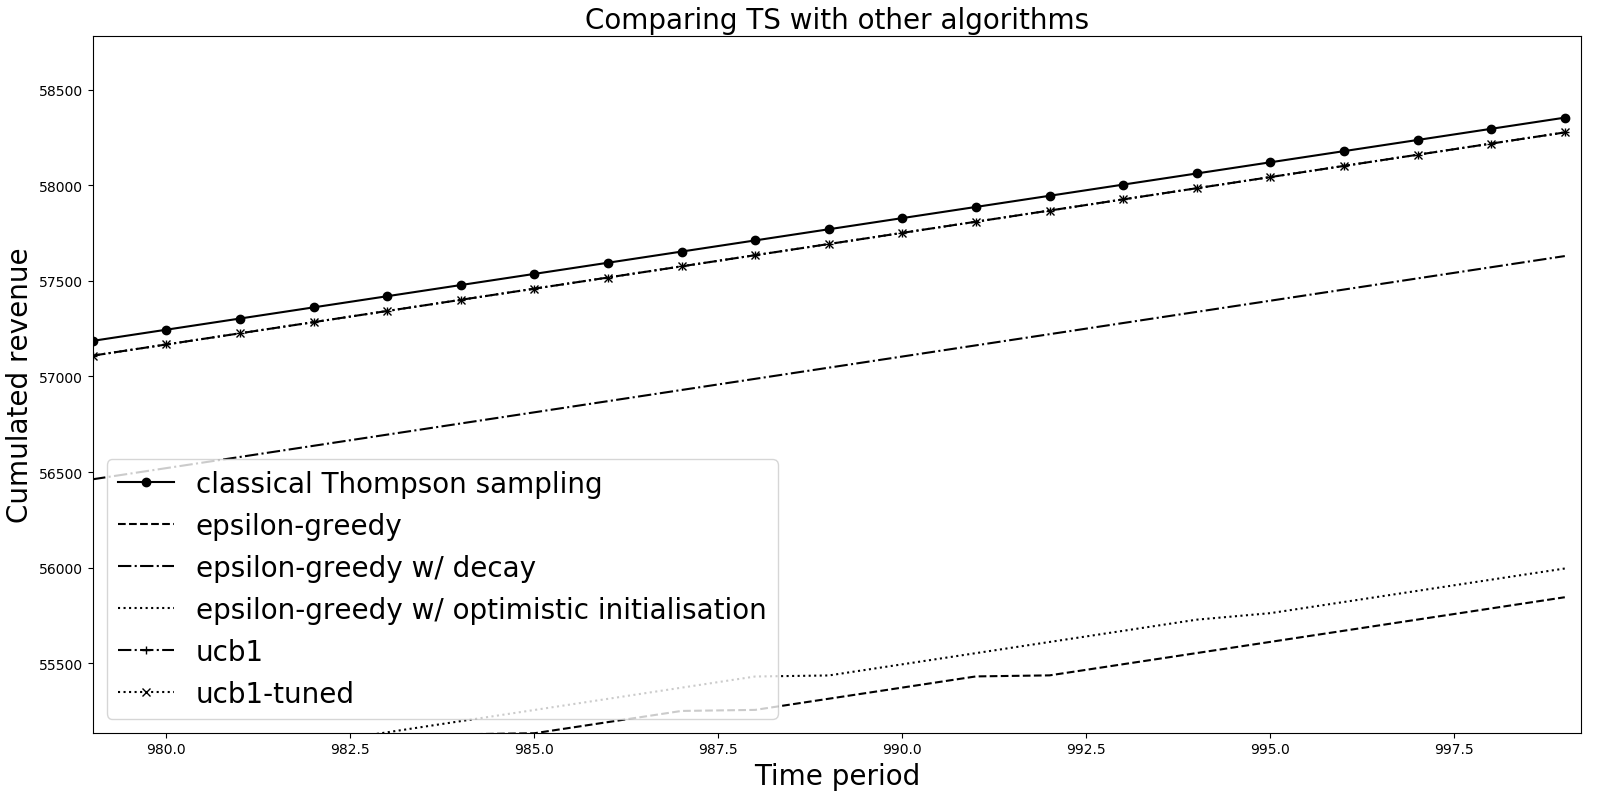
\includegraphics[width=1\textwidth]{Figure_1-4.png}
	\caption{\label{fig:three}Comparing revenue between all algorithms - last 20 time periods}
\end{figure}
\pagebreak
\section{Second approach}
In this approach, the objective is to learn the true elasticity values for each product. We implement the Thompson Sampling algorithm for dynamic pricing proposed by Ganti, Sustik, Tran \& Seaman (2018). In their paper, they consider the demand function to be a modified constant elasticity model. The commonly used constant elasticity model is 
\[d_i(p_i) = f_i \left(\frac{p_i}{p_{0,i}}\right)^{\gamma_{*,i}} \]
where $d_i(p_i)$ is the demand of item $i$ at price $p_{0,i}, f_i$ is the baseline demand at price $p_{0,i}$ for item $i$ and $\gamma_{*,i} < -1$ is the elasticity of item $i$. Instead of this model, the authors proposed 
\[d_{i,t}(p_i) = f_{i,t} \left(\frac{p_i}{p_{i,t-1}}\right)^{\gamma_{*,i}} \]
which we will implement for this approach. $f_{i,t}$ is the demand forecast for item $i$ on day $t$ if the price is $p_{i,t-1}$. This has several advantages over the MNL model and the typical constant elasticity model. Firstly, the demand function in real world pricing systems is usually not stationary and the adaptations made can reflect this property by accounting for possible movements in the underlying demand function. Secondly, the MNL model assumes homogeneous customer behaviour i.e every customer has the same purchasing behaviour. On the other hand, the constant elasticity model is an aggregate model i.e the model perceives the market as a whole and not as one customer. This may be more similar to real world pricing systems.
\newline
\newline
In this section, we will compare the results of the dynamic pricing algorithm to a model with no dynamic pricing implemented, which we will call the constant price model. The comparison will be done in two settings - one with inventory constraint and the other without inventory constraint.
\newline
\newline
The dynamic pricing algorithm needs a prior distribution $\Pi_0(\gamma_*)$ which is assumed to be a normal distribution for the elasticity and an estimate for the noise variance $\sigma^2$. The authors suggest using prior elasticity estimates from historical data as the mean $\mu_0$ of the prior distribution and $\Sigma_0 = cI$ for some constant c as the covariance matrix. Similarly, sample standard deviation of observed revenue from historical data can be used to estimate $\sigma$. In our implementation, since Thompson sampling learns the true parameter values over time, we randomly initialised $\mu_0 \in [-5, -1]^{66}$ and set $c$ to be 10\% of the mean of $\mu_0$. Even if the initialisation choice was poor, TS will still be able to learn the true values albeit taking a longer period of time. From our dataset, there were 2 days in which all products had at least 1 sale. $\hat{\sigma}$ was set to be the standard deviation of the observed revenue for those two days. Here is how the algorithm proceeded:
\newline
\newline
Set the true elasticity $\gamma_*$ to be some random vector where $\gamma_* \in [-3, -1]^{66}$ and this is not revealed to the algorithm. This is a reasonable assumption since the products in the dataset are children's books, which are usually elastic in demand. Set $\beta=0.5$, $p_{i,0}$ to be the actual price from the dataset and $d_{i,0}$ to be one of the eleven days from the dataset. By fixing $d_{i,0}$, the starting point of the algorithm is fixed. We may then compare performance across different models. $\epsilon_t$ is random noise sampled independently from $N(0,1)$. $T$ was chosen to be 15 in this section since sales promotions are usually not that long in real world pricing systems
\newline
\newline
For iterations $t = 1,...,T$, the following process was done for the dynamic pricing algorithm:
\begin{enumerate}
	\item Calculate demand forecast for each item $i$ using the autoregressive model \[ f_{i,t} = c_0 + \sum_{\tau=t-1}^{0} \beta^{t-\tau}d_{i,\tau} + \epsilon_t \]
	\item Randomly sample from $\gamma_t \sim \Pi_{t-1}$ until all components of $\gamma_t$ are negative since elasticity values are negative.
	\item Solve the following optimisation problem to get price vector $p_t$ given $p_{i,t-1}$ and estimates $f_{i,t}$ and $\gamma_t$ \[p_t = \argmax_p \sum_{i=1}^{N}\frac{p_i^2f_{i,t}\gamma_{*,i}}{p_{i,t-1}} -p_if_{i,t}\gamma_{*,i} + p_if_{i,t}\] \[\text{subject to: } p \in C_t \]
	\item Apply prices $p_t$. The observed demand is generated by the following modified constant elasticity formula \[ d_{i,t}(p_{i,t}) = \text{max} \left(f_{i,t}\left(\frac{p_{i,t}}{p_{i,t-1}}\right)^{\gamma_*} + \epsilon_t, 0 \right) \] 
	\item Update our prior distribution $\Pi_{t-1}(\gamma_*)$ to obtain the posterior distribution $\Pi_t(\gamma_*)$. The details of Bayes updating in this step can be found in  Ganti, Sustik, Tran \& Seaman (2018)'s paper - equations (16) and (17).
\end{enumerate}
For the constant price model, the price $p_t$ was set as $p_{i,0}$ in every iteration. Steps 2, 3 and 5 were also removed since we do not implement any learning algorithms. We are interested to investigate if applying dynamic pricing would lead to better results over not applying any algorithms.
\subsection{Dynamic vs Constant pricing without constraint}
In this subsection, we do not impose any constraint and simply implement the algorithm proposed by the authors on the real dataset.
\begin{figure}[h]
	\centering
	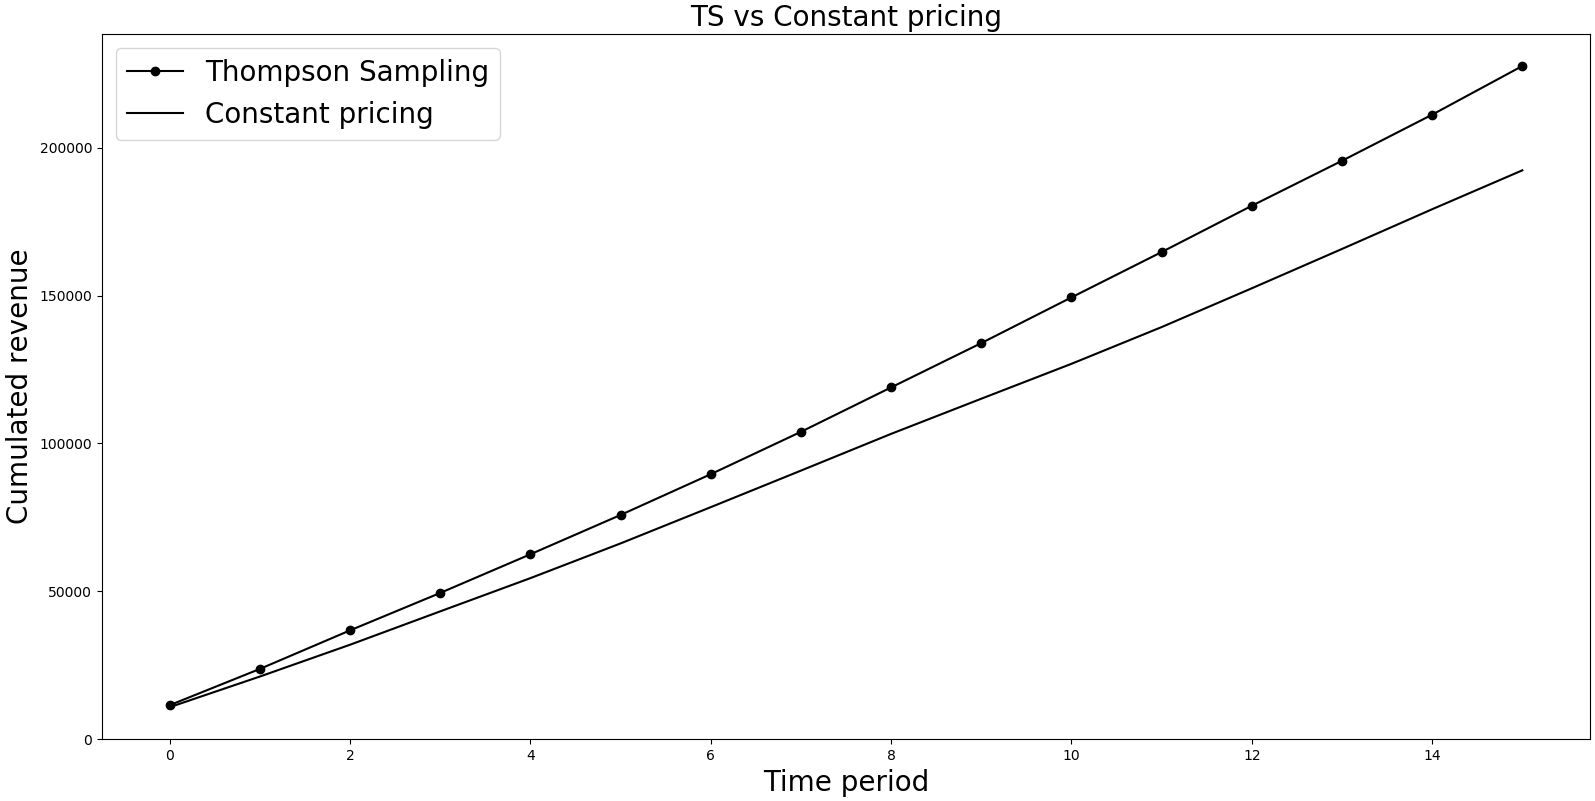
\includegraphics[width=1\textwidth]{Figure_2-1.png}
	\caption{\label{fig:four}Comparing cumulated revenue between TS and constant pricing without inventory constraints}
\end{figure}
\newline
Since we do not impose any inventory constraint, it is assumed that the seller has sufficient stock to satisfy demand in each time period. In each successive time period, the price of products fall gradually while demand increases steadily. As the products are elastic in demand, the decrease in prices leads to a larger increase in demand which results in higher revenue.
\newline
\newline
By the end of the horizon, TS earned 14.8\% more revenue than the constant pricing model and also sold 65.8\% more products. If we had 1000 of each product in inventory at the beginning of the selling season, we can also analyse the amount of inventory cleared. In most real world situations, products may no longer be sold after the selling season is over and there is a cost accrued by the seller for not being able to sell it. We can assign a cost to each product and investigate the total costs for each model. By setting cost $= 0.5  p_{i,0}$ and taking into account the amount of products left over, TS had incurred 15.5\% less costs than the constant pricing model. On the whole, TS made 21.5\% less losses where loss = costs - revenue.
\newline
\newline
We can frame this problem as trying to clear excess inventory during a finite selling season (15 time periods) and the decrease in prices as coupons offered to customers. Even though the main objective is to clear inventory, we also want to ensure that we are able to minimise losses and maximise profits as much as possible. Thus, when assuming no inventory constraints (the seller is able to meet the market's demand in every time period) and the independence of products' elasticities, the dynamic pricing algorithm works better.
\subsection{Dynamic vs Constant pricing with constraint}
In this subsection, we explicitly set the amount of inventory to be 50 and not 1000 as in the previous section as we are interested in how the algorithms perform when there is no more inventory. The algorithms will continue until all inventory has been cleared. More specifically, we subtract the observed demand in each iteration from a finite amount of inventory. When a product has run out of inventory, we set the observed demand in step 4 of the algorithm to be 0 for that product for all subsequent time periods.
\begin{figure}[h]
	\centering
	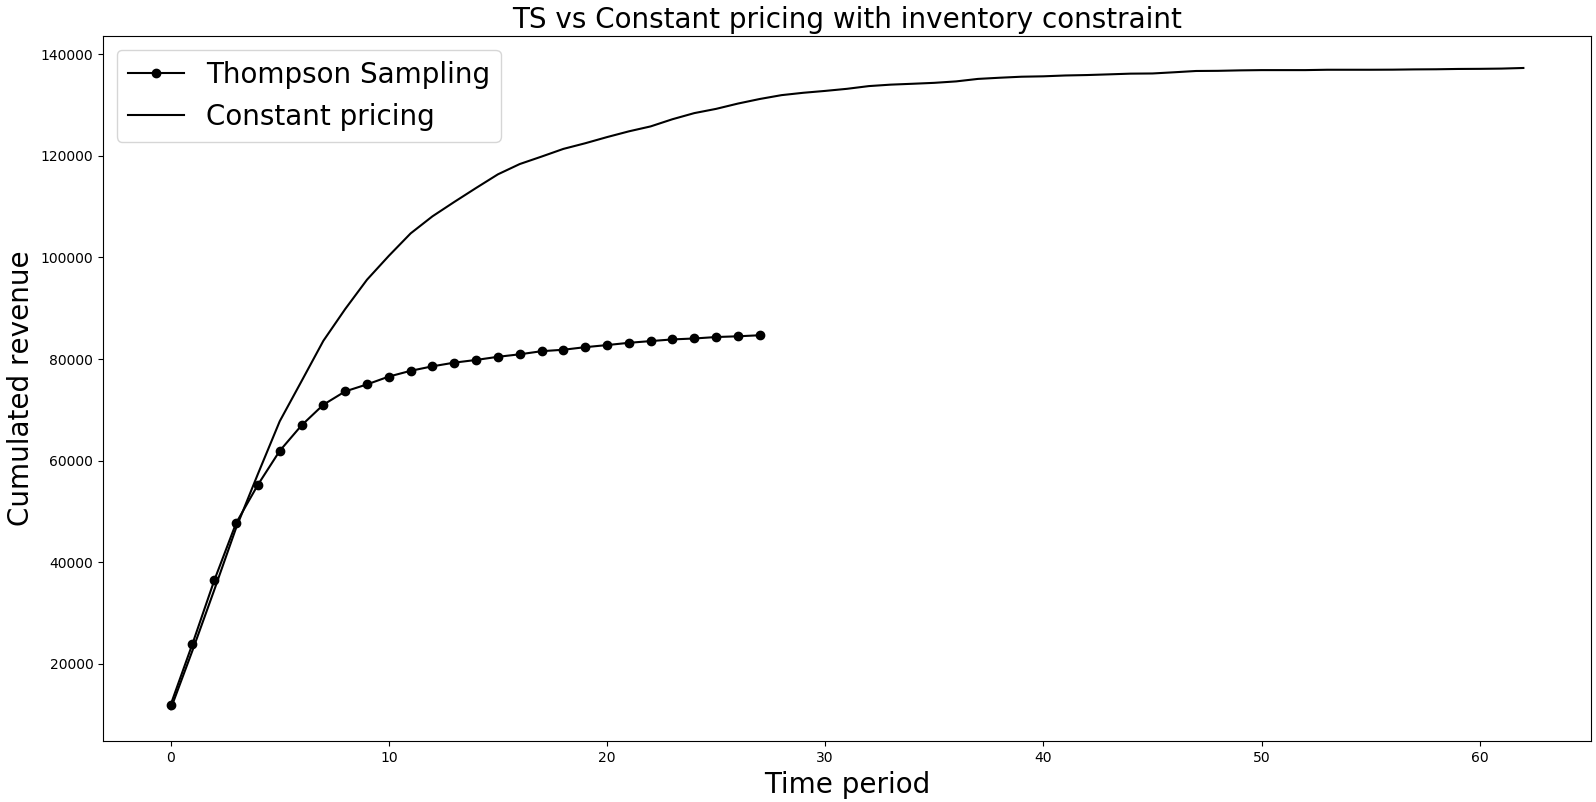
\includegraphics[width=1\textwidth]{Figure_2-2.png}
	\caption{\label{fig:five}Cumulated revenue of TS and constant pricing with inventory constraints}
\end{figure}
\newline
\newline
As seen in Figure \ref{fig:five}, TS clears the inventory much quicker than the constant pricing model. However, the amount of revenue generated by TS is significantly lower. As explained in the previous subsection, the TS algorithm increases revenue by lowering prices which will lead to an increase in demand since the products' demand is elastic. This is not reflected in Figure \ref{fig:five} and we believe the reason may be due to the fact that most of the products have already run out of inventory. 
\newline
\newline
If we repeat our approach in the previous subsection by cutting off the plots at time period = 15, the constant pricing model earned 30.9\% more revenue than TS but incurred 45.3\% more costs. It also sold 8.5\% less products than TS but still managed to record 29.6\% more profits where profits = revenue - costs. Thus, the decrease in prices is not compensated by the increase in demand as there is simply insufficient stock to meet the market's demand. This further reinforces our assumption from the previous subsection that the seller should be able to meet the market's demand in each time period. It may be difficult to observe from Figure \ref{fig:five} but between the second and fourth points, the revenue by TS is actually greater than the revenue by the constant pricing model and it closely resembles the plot in Figure \ref{fig:four}. After the fourth point, the plot of TS starts to taper off. This is due to inventory running out and thus the observed demand for most products is 0.


\section{Conclusion and future direction}
In this paper, we explored the algorithm known as Thompson sampling in various settings. We compared its performance to other well-known algorithms such as UCB in the MAB problem using a MNL demand function with synthetic data. We observed that TS greatly outperformed greedy algorithms and to a smaller extent, UCB algorithms which are considered to be more commonly utilised. 
\newline
\newline
We then implemented a dynamic pricing algorithm using Thompson sampling proposed by Ganti, Sustik, Tran \& Seaman (2018) on a real dataset which consisted of sales data of children's books. In this approach, instead of the MNL model, we used a modified constant elasticity model as the demand function. We compared its performance to a constant pricing model in two different settings: with inventory constraint and without inventory constraint. In the setting  without inventory constraint, Thompson sampling easily outperforms the constant pricing algorithm. It achieves higher revenue at less cost and is able to sell more products which led to smaller loss than the constant pricing algorithm. In the setting with inventory constraints, we set the observed demand of products with depleted stock to be 0. As a result, the constant pricing model outperforms TS by tapering off much later. We believe this is due to the decrease in product prices not being sufficiently compensated by the increase in demand as there is simply no stock left. Thus, a required assumption of the dynamic pricing algorithm with TS is that the seller must be able to meet customers' demand in the entire horizon.
\newline
\newline
As we saw in the second approach, the dynamic pricing algorithm with TS fails when inventory constraints are introduced and only succeeds when the seller knows they can meet market demand during the selling season. In certain real world markets, this may not be a very flexible assumption since demand may change overtime due to external events. A seller might be in the middle of the selling season when he realises his supply is insufficient due to changes in the market. He will then have to cease TS or risk incurring losses. It may thus be worthwhile to investigate extending this dynamic pricing algorithm with TS to be more robust against inventory constraints. A possible direction would be to incorporate inventory constraints more elegantly instead of setting observed demand to be simply 0. A good resource to start with would be Ferreira, Simchi-Levi \& Wang (2017)'s paper where they investigate different products requiring different kinds of resources in detail.
\newpage

\begin{thebibliography}{9}
	\bibitem{nano3}
	https://www.statista.com/statistics/534123/e-commerce-share-of-retail-sales-worldwide/
	
	\bibitem{CK}
	https://milled.com/CalvinKlein/final-hours-take-40-off-every-100-spent-Q2RTJAp7mfdfwq3I
	
	\bibitem{1}
	Araman, V. F., R. Caldentey. 2009. Dynamic pricing for nonperishable products with demand learning.
	\emph{Operations Research} 57(5) 1169-1188.
	
	\bibitem{1a}
	Aviv, Yossi and Pazgal, Amit. 2005. A partially observed markov decision process for dynamic
	pricing. \emph{Management Science} 51(9) 1400–1416.
	
	\bibitem{bada}
	Badanidiyuru, A., R. Kleinberg, A. Slivkins. 2013. Bandits with knapsacks. \emph{IEEE 54th Annual Symposium on Foundations of Computer Science (FOCS).} 207-216.	
	
	\bibitem{brod}
	Broder, Josef and Rusmevichientong, Paat. 2012. Dynamic pricing under a general parametric choice model. \emph{Operations Research} 60(4) 965-980.
	
	\bibitem{bub}
	Bubeck, S., N. Cesa-Bianchi. 2012. Regret analysis of stochastic and nonstochastic multi-armed bandit problems. \emph{Foundations and Trends in Machine Learning} 5(1) 1-122.
	
	\bibitem{thomp}
	Chapelle,  Li. 2011. An Empirical Evaluation of Thompson Sampling. NIPS. 
	
	\bibitem{2}
	Farias, V., B. Van Roy. 2010. Dynamic pricing with a prior on market response. \emph{Operations Research} 58(1) 16-29.
	
	\bibitem{inventory}
	Ferreira, Simchi-Levi, Wang. 2017. Online Network Revenue Management Using Thompson Sampling. \emph{Operations Research}
	
	\bibitem{main}
	Ganti, Sustik, Tran, Seaman. 2018. Thompson Sampling for Dynamic Pricing. 
\end{thebibliography}

\end{document}